\section{Neural Networks}\label{sec:NN}
The concept of a \ac{NN} has been around for more than 80 years, and today they are one 
of the most popular and successful \ac{ML} methods. The key to its popularity stems from
its versatility, achieving high performance in a large range of both regression 
and classification problems. One of the defining qualities in a \ac{NN} is the 
possibility of diverse architecture, meaning that a there are many
categorize of \ac{NN}, where each category has an even deeper selection of
networks. Categories ranging from \ac{CNN}, \ac{RNN} to simple \ac{FFNN}, where each
category is specified for their own set of problems. In this section I will introduce 
some fundamental definitions in regard to \ac{NN}, as well go through the underlying 
algorithm of the back- and forward propagation.

\subsection{General structure}
There are often drawn comparisons between the structure of the neural network, 
and the way the human mind operate, hence neural. Similarly to the human mind, a \ac{NN} is 
composed of different neurons communicating information backwards and forwards in different 
regions In the case of a neural network we call these regions layers. All layers
are composed of a specified number of neurons. A \ac{NN} has three types of layers;
\emph{input-layer}, \emph{hidden-layer} and \emph{output-layer}. There is only one input layer, and it has
the same number of nodes equal to the number of features for each data point. 
There can be an arbitrary number of hidden layers, with each hidden-layer containing
an arbitrary number of nodes. Finally, the \ac{NN} has an output layer. The output-layer
contains a number of nodes equal to the number of features for the target.
\\
The neural network functions by passing information in between the different layers though 
nodes. The nodes are simply pockets of information, each containing a value. 
All the nodes in the input layer are (in most cases) connected to all nodes in the nearest hidden layer,
and likewise said hidden layer is connected to the next hidden layer. This structure continues
until we reach the final layer, the output layer. The structure is illustrated in figure
\ref{fig:NN}. The figure shows a simple \ac{NN} with a 2 dimensional data set (2 nodes in input-layer),
2 hidden layers with three nodes each and a 1 dimensional target value. It also illustrates 
how a \ac{NN} aims to map from data, $\x$ to a prediction $\y$.
\begin{figure}
    \centering
    \vspace*{-12.5mm} 
    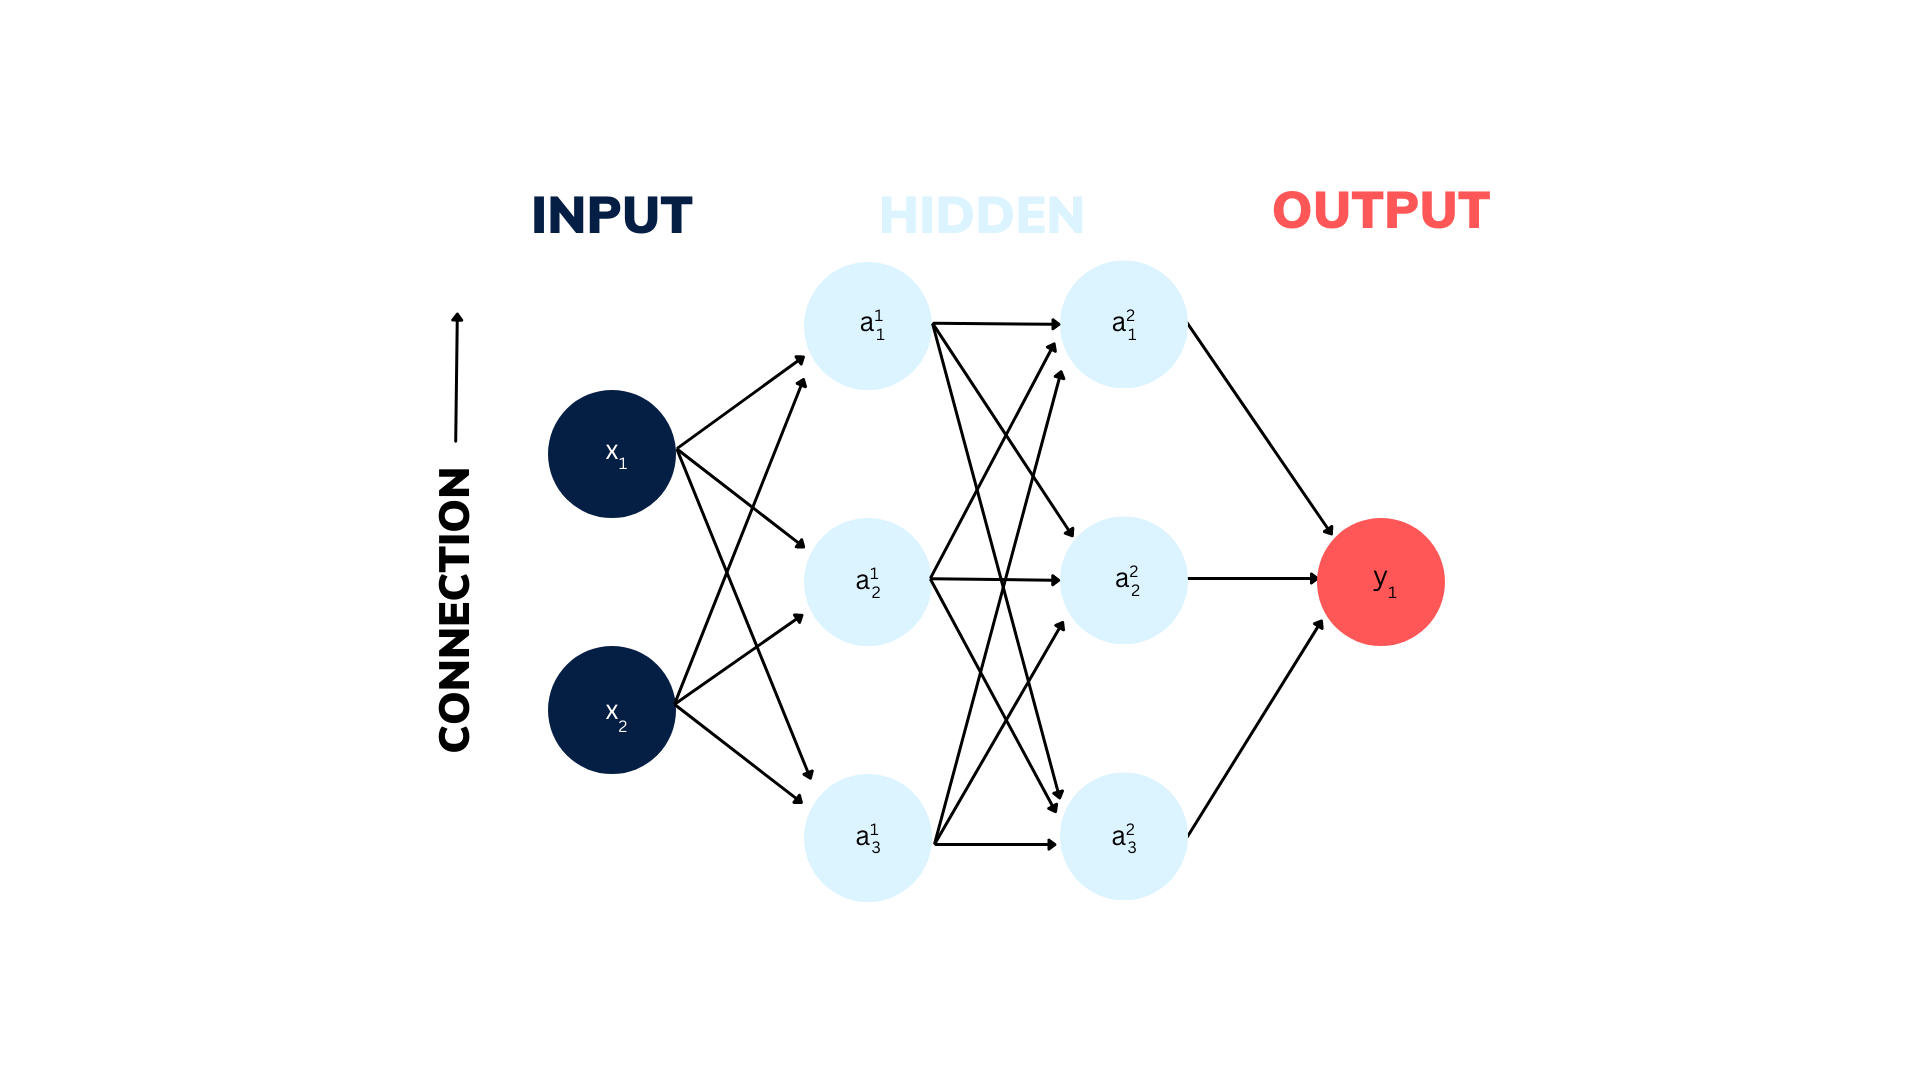
\includegraphics[width=0.9\textwidth]{Figures/Illustrations/Input_labels.png}
    \vspace*{-12.5mm} 
    \caption{An illustration of a \ac{NN} with two hidden layers.}
    \label{fig:NN}
\end{figure}
In figure \ref{fig:NN} we can see how all the different nodes are connected, illustrated by 
the arrows. The passing of values between different nodes are controlled by a set of weights and
bias parameters. These parameters are defined for each connection and are what will be tuned 
during training. The weights and biases for a given connection of two nodes, defines the effect on node 
has on the other.
\\
In a traditional \ac{FFNN} the information is passed linearly (in figure \ref{fig:NN}, from left to right) 
in a process we call \emph{forward-propogation}. Other variants can include the information taking a more 
complex route. It is often the route from input- to output-layer that categorizes the type of \ac{NN}. In 
this report I used a simple \ac{FFNN}. 

\subsection{Feeding Forward}\label{subsec:FP}
With the structure described in the previous section, a trained model, $\mathcal{F}$ produces a prediction,
$\{\textbf{y}\}_{i=0}^N$ for a data set, $\{\textbf{x}\}_{i=0}^N$, where N is the dimensions of the input, by passing information 
from input-layer, through all hidden-layers then to output-layer, which we call forward-propagation. In this section 
I aim to explain the underlying algorithm and math used by the \ac{NN} to map input to output. 
\\
We imagine the passing from hidden-layer $l-1$ to $l$, where $l \in \{2,...,L \}$\footnote{There is a special
case for when $l=1$ which will be addressed in the next paragraphs.} and $L$ is equal to the
number of hidden layers. The value of a node in layer $l$, is defined as $a^l_j$ (as indicated by figure \ref{fig:NN}), 
where $j\in \{0,1,...,N_l\}$ and $N_l$ is equal to the number of nodes in $l$. The value of $a_j^l$ is defined as 
the \emph{activated} sum of all nodes in the previous layer, $a_j^{l-1}$ where the sum is weighted by a parameter $\bf{w} \sf _j^l$ 
and scaled by the bias, $b^l_j$ for $j\in \{0,1,..., N_{l-1} \}$. The inactivated value of for a node j in layer l is defined as 
\begin{align}\label{eq:activated}
    z_j^l = \sum_{k=1} ^ {N_{l-1}} w_{kj}^la_k^{l-1} + b^l_k,
\end{align}
where $w_{kj}^l$ corresponds to the weight in $\bf{w} \sf _k^l$ specific for the connection between node k and j.
\\
To attain the full activated value, $a_j^l$ we pass $z_j^l$ through the \emph{activation function}. The activation function, $\sigma^l$ 
is a generally non-linear function used to control the limit or expand the value range for the node values. The activation 
function is general for all nodes in a given layer, but can vary in between layers. Therefore,
we find $a_j^l$ by the equation
\begin{align}\label{eq:ajl}
    a_j^l = \sigma \left (\sum_{k=1} ^ {N_{l}} w_{kj}^la_k^{l-1} + b^l_k\right ) = \sigma^l(z_j^l).
\end{align}
A more detailed illustration of the information pass from one layer to a node in the next is displayed 
in figure \ref{fig:WB}. In figure \ref{fig:WB}, we see all steps described in the process; \emph{(1)} all nodes in 
l-1 are summed with a corresponding weight, \emph{(2)} the sum is scaled by a constant term (bias), \emph{(3)} the 
scaled and weighted sum defines the inactivated value $z_j^l$, \emph{(4)} we define $a^l_j$ by passing the 
sum through $\sigma^l$.  
\begin{figure}
    \centering
    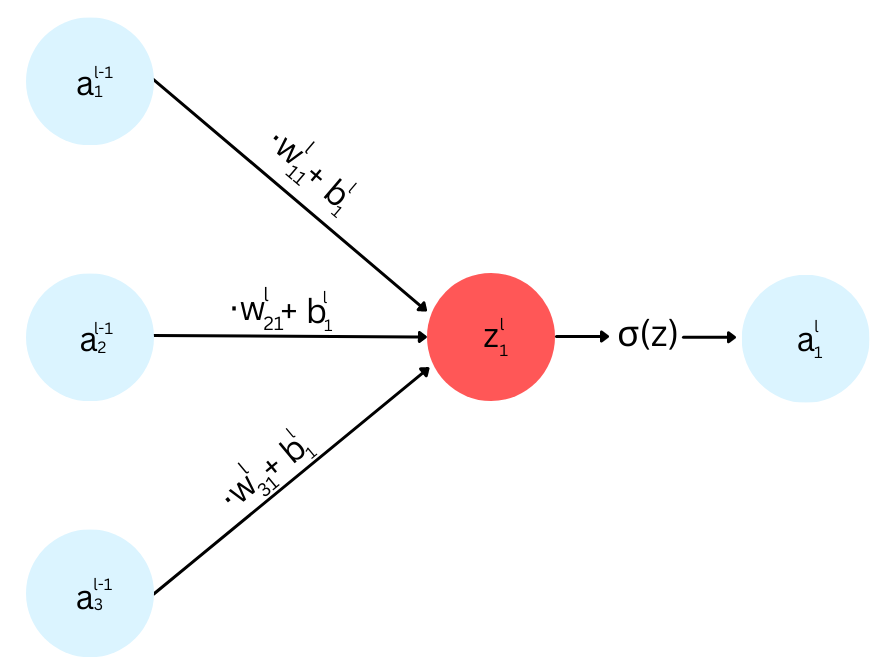
\includegraphics[width=0.5\textwidth]{Figures/Illustrations/WeightBias.png}
    \caption{An illustration information pass for one layer to another.}
    \label{fig:WB}
\end{figure}
This method is used for information pass between all layers, except the between the first and the second. 
In this case we simply replace the activated term, $a_k^{l-1}$ in equation \ref{eq:ajl}, by the input data,
$x_i$ for $i\in\{0,1,...,N\}$, where N is equal to the number features for the data. In the case $l=1$, \ref{eq:ajl} 
becomes
\begin{align}
    a_j^1 = \sigma \left (\sum_{k=1} ^ {N} w_{kj}^1x_k + b^1_k\right ) = \sigma(z_j^1).
\end{align}
And in the case where $l=L$, $a_j^L$ is equal to the final output. 
\subsection{Back Propagation}\label{subsec:BP}
The backward propagation acts as the engine that drives the training of a neural network. It has the purpose
of tuning the weights and biases of the network to achieve maximum performance, as defined by some 
\emph{cost function}, $\mathcal{C}$. The cost function defines to which metric we aim to optimize the network. 
In the case a neural network produces a prediction, $\y$ which aims to recreate a target $\ti$ the error in the prediction
is defined by the cost function as $\mathcal{C}\left(\y, \ti\right)$. To minimize $\mathcal{C}$, the 
backwards propagation utilizes the gradient with respect to the weights and biases in the network. Instead of a
direct calculation of the gradient, which is very computationally heavy, the backward propagation 
aims to calculate the gradient through a recursive algorithm which traces the error backwards through the network. It is 
this algorithm I will describe in this section.
\\
\newline
When minimizing the error defined by $\mathcal{C}$, we can apply several optimization algorithms described in 
section \ref{sec:Opti}. Common for the algorithms is the use of the gradient of the cost function with regard to 
the tunable parameters. In our case these parameters are the weights and biases, $w_{k,j}^l$ and $b^l_k$. The goal of 
the backwards propagation is therefore to calculate the gradients $\partial \mathcal{C}/\partial w_{k,j}^l$ and
$\partial \mathcal{C}/\partial b^l_k$. 
\\
\newline
To begin with we can derive an expression for $\partial \mathcal{C}/\partial w_{k,j}^l$. We use the chain-rule to define 
\begin{align*}
    \frac{\partial \mathcal{C}}{\partial w_{k,j}^l} = \frac{\partial \mathcal{C}}{\partial z^l_k} \frac{\partial z^l_k}{\partial w_{k,j}^l},
\end{align*}
which we can simplify further by using equation \ref{eq:activated} to calculate the second term, which becomes
\begin{align*}
    \frac{\partial \mathcal{C}}{\partial w_{k,j}^l} = \frac{\partial \mathcal{C}}{\partial z^l_k} a^{l-1}_j.
\end{align*}
We can redefine the first term in the equation above as $\delta_j^l$ and write
\begin{align*}
    \delta_k^l = \frac{\partial \mathcal{C}}{\partial z^l_k}
               = \sum_j \frac{\partial \mathcal{C}}{\partial z^{l+1}_j}\frac{\partial z_j^{l+1}}{\partial z^l_k}  
               = \sum_j \delta_k^{l+1}\frac{\partial z_j^{l+1}}{\partial z^l_k},
\end{align*}
where we have again used the chain rule for all contributing nodes.
\\
To calculate the final partial derivative we write
\begin{align*}
    \frac{\partial z_j^{l+1}}{\partial z^l_k} = \frac{\partial z_j^{l+1}}{\partial a^l_j}\frac{\partial a^l_j}{\partial z^l_k}
                                              = w_{jk}^{l+1}(\sigma^l(z_j^l))'.
\end{align*}
This gives use the expression for $\delta_j^l$
\begin{align}\label{eq:delta}
    \delta_k^l  = \sum_k \delta_k^{l+1}w_{jk}^{l+1}(\sigma^l(z_j^l))'  
\end{align}
Finally this gives us the expression
\begin{align}\label{eq:dw}
    \frac{\partial \mathcal{C}}{\partial w_{k,j}^l} = \delta_k^{l} a_j^{l-1}.
\end{align}
Next we want to derive $\partial \mathcal{C}/\partial b^l_k$. We simply use the chain rule and derive
\begin{align*}
    \frac{\partial \mathcal{C}}{\partial b^l_k} = \frac{\partial \mathcal{C}}{\partial z^l_k}\frac{\partial z_k^l}{\partial b^l_k},
\end{align*}
which from equations \ref{eq:delta} and \ref{eq:dw} is simply
\begin{align}\label{eq:db}
    \frac{\partial \mathcal{C}}{\partial b^l_k} = \delta_k^{l} \cdot 1 = \delta_k^{l},
\end{align}
From all three derived expressions, equations \ref{eq:delta}, \ref{eq:dw} and \ref{eq:db} we see that 
to calculate for all $l\in\{0,1,..,N_l\}$ we must first calculate $\delta_k^L$ and apply a recursive propagation.
To calculate $\delta_k^L = \partial \mathcal{C}/\partial z^L_k$ we simply multiply by $\delta_k^L = \partial a_k^L/\partial a_k^L$, and we find
\begin{align}\label{eq:deltaL}
    \delta_k^L = \frac{\partial \mathcal{C}}{\partial a^L_k}\left(\sigma^L(z_k^L)\right)'
\end{align}
This expression, similarly to equation \ref{eq:delta} is dependent on the choice of $\mathcal{C}$ and 
the activation functions. Now that equation \ref{eq:deltaL} is defined, we can see that the
gradient of the parameters in all other layers can be calculated. 

\subsection{Activation functions}
As mentioned in previous sections, activation functions define how the nodes in the previous layer 
sum to define the value of the node in the current. There are many types of activation functions, 
where all have advantages and disadvantages. The choice of activation function for each layer is defined
before training, making it a hyperparameter. The activation functions applied and tested in this thesis are the following:
\begin{center}
\begin{itemize}
    \item  \emph{Sigmoid}\\  
    \begin{align*}
         \sigma{(z)} = \frac{1}{1+e^{-z}} = a \in [0,1]
    \end{align*},
    \item \emph{Leaky ReLU}
    \begin{align*}
        \sigma{(z)} = 
        \begin{cases}
            z,& \text{if } z\geq 0\\
            \mu z,              & \text{otherwise}
        \end{cases}
        = a \in (-\infty, \infty),
   \end{align*}
   where $\mu$ is scalar.
\end{itemize},
\end{center}
where $z$ is an inactivated node which is activated to define $a$, the activation.

\subsection{Network Ensembles, dropout and LWTA networks}
So far in the thesis, I have only covered dense layers, meaning that every node in the layer before it is 
connected to its own nodes and likewise all its nodes are connected to the nodes in the layer that follows. 
This definition covers many, but not all hidden layer. Some layers do not function to pass value to and 
fro between nodes but instead functions by dynamically changing the architecture of the \ac{NN}. The most popular 
type of layer that fits this definition, is the \emph{dropout}-layer. The dropout-layer functions by randomly 
choosing a predetermined number of neurons in the layer before it, and dropping them from the network for the current 
round of training. By doing this the dropout-layer creates an architecture for the network for every round
of training. Each unique architecture represents its own network in what becomes an ensemble of networks. 
\\
As mentioned in previous sections, creating ensembles of models is a form of regularization. In the case of 
dropout, it minimizes the risk of overfitting by hindering a phenomenon known as complex co-adaptations. Complex
co-adaptation happens when a neuron becomes overly dominant such that neighboring neurons no longer contribute (relative
to the dominant neuron) and therefore lack the motivation to tune. When this happens, networks become fragile and overly 
specialized to the training data. By randomly dropping neurons, the neighboring neurons are no longer allowed to be passive 
and are forced to tune to compensate. During evaluation, the dropout layers no longer take action. Instead, the dropout rate 
(fraction of neurons to drop in the layer) $r$ is used to scale the weights by a factor $1-r$. The prediction made by the resulting 
model can therefore be seen as the average of all the smaller networks. In other words, a neural network containing dropout-layers 
as a bagging ensemble. 
\\
Dropout-layers are not the only layers to dynamically change the architecture of a network. In this thesis I additionally 
explored the lesser known, \emph{max-out}-layer. Max-out, similarly to dropout creates an ensemble of networks by removing a set 
of nodes for each round of training. Contrary to dropout, max-out does not choose the nodes to drop at random,
but instead creates local units by grouping the nodes, and removes all nodes except the node with the largest
activation. The goal of max-out is to create an ensemble of networks where each network is specialized for a given 
trend in the data. In this thesis I have implemented the layer such that upon prediction, the redimensionalization 
is still active. This means that for each data point, a neural network is chosen based on the specific activations in 
each of the nodes. In other words, the max-out layer creates something resembling a stacking ensemble. 
\\
In figure \ref{fig:Max_out} I have illustrated a max-out network. The figure shows a \ac{NN} with two hidden layers
with 8 nodes each. In the first hidden layer the max-out layer creates 4 units, each containing two nodes and in the 
second layer the max-out creates two nodes with 4 nodes each. The resulting output from the first layer is the 
4 nodes with the highest activation in their respected unit, likewise the second layers output is 2 nodes.
To the right of the network in figure \ref{fig:Max_out}, I have illustrated how the different configuration of 
paths through the network creates an ensemble of networks with their own architecture.
\begin{figure}
    \centering
    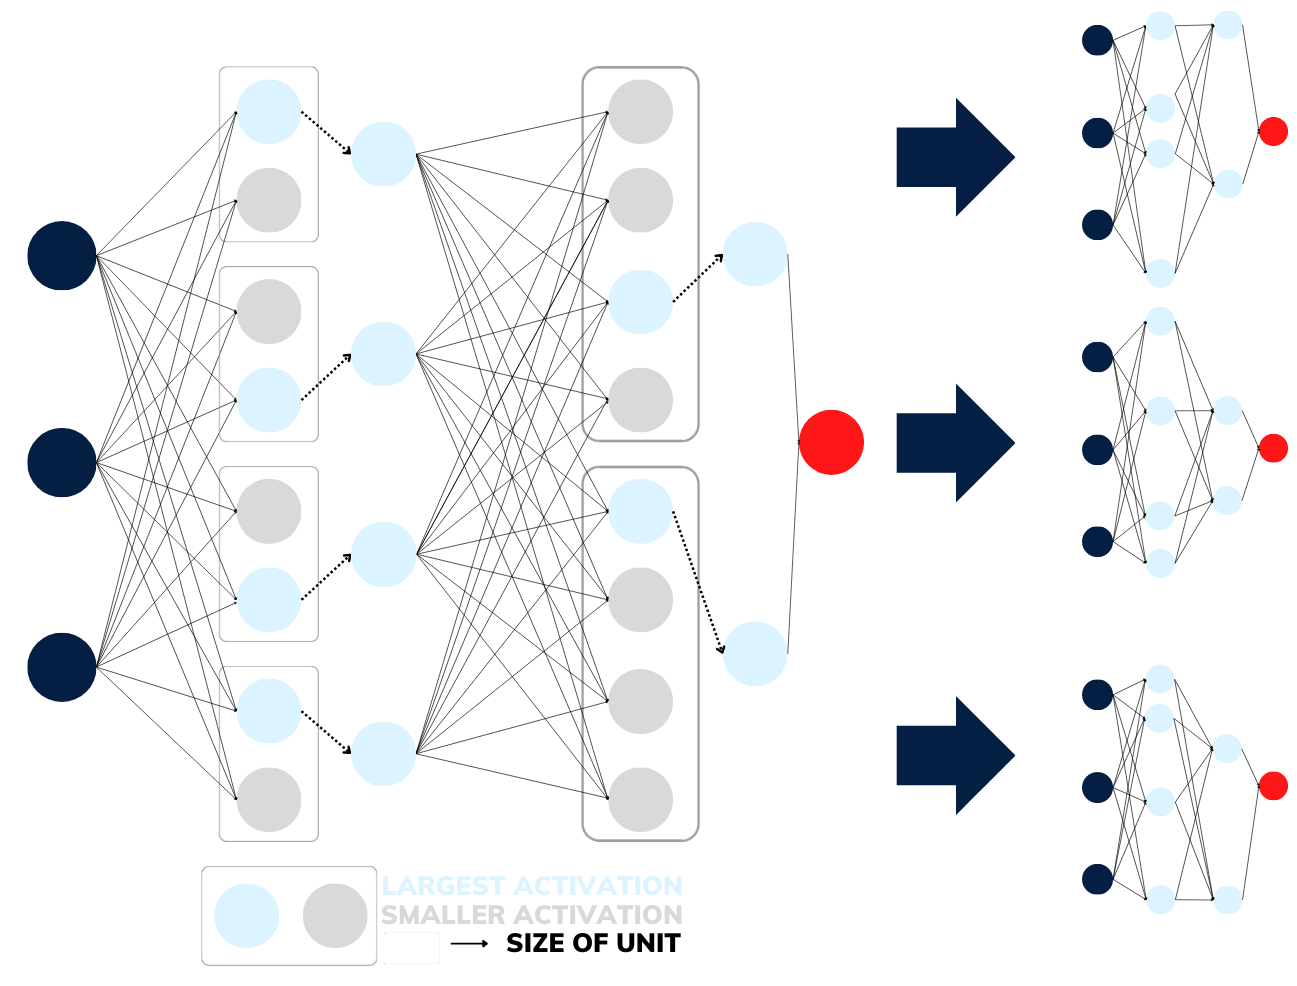
\includegraphics[width=0.7\textwidth]{Figures/Illustrations/Max_out.png}
    \caption{An illustration of a Neural network with two hidden layers, each with 8 neurons.
    The first hidden layer has a max-out activation layer with 4 units, the second has 2.
    The figure also illustrates  the resulting ensemble of smaller neural networks as a consequence
    of the max-out activation layers. }
    \label{fig:Max_out}
\end{figure}






